\documentclass[12pt,a4paper]{article}
\usepackage[
type={CC},
modifier={by-nd},
version={4.0},
]{doclicense}

\usepackage[utf8]{inputenc}
\usepackage[T1]{fontenc}
\usepackage{amsmath}
\usepackage{amssymb}
\usepackage{graphicx}
\usepackage[french]{babel}
\usepackage[a4paper]{geometry}
\geometry{top=20mm,bottom=15mm,inner=15mm,outer=10mm}
\DeclareUnicodeCharacter{000B}{}
\usepackage{listings}
\lstset{language=C,basicstyle=\ttfamily}
\usepackage{hyperref}
\usepackage{makeidx}
\makeindex
\setlength{\parskip}{0.2em}

\newcommand{\rep}[1]{\fbox{$#1$}}

% ===============================
% TITRE
% ===============================

\title{Group 3 -- User Guide \textit{SoundWay}}
\author{Esteban BARRACHO\\
        Anas DAMLAKHI\\
        Jonathan KONDOLI NKEBI\\
        Arthur SMOOS\\
        Bénédicte TUTEKA MUKUTA}

% ===============================
\begin{document}
% ===============================

\maketitle
\thispagestyle{empty}
\vspace*{18em}

\begin{center}
    
\includegraphics[width=0.25\textwidth]{figures/LogoUNamur.jpg}\\[0.5em]
    University of Namur -- Faculty of Computer Science
\end{center}
\newpage

\begin{center}
    \textbf{SoundWay}\\[0.5em]
    BLE multi-advertising system with voice interaction and mobile feedback\\
    for indoor orientation assistance
\end{center}

\vspace*{2em}

% ======= LOGO DE L’APPLICATION =======
\begin{center}
    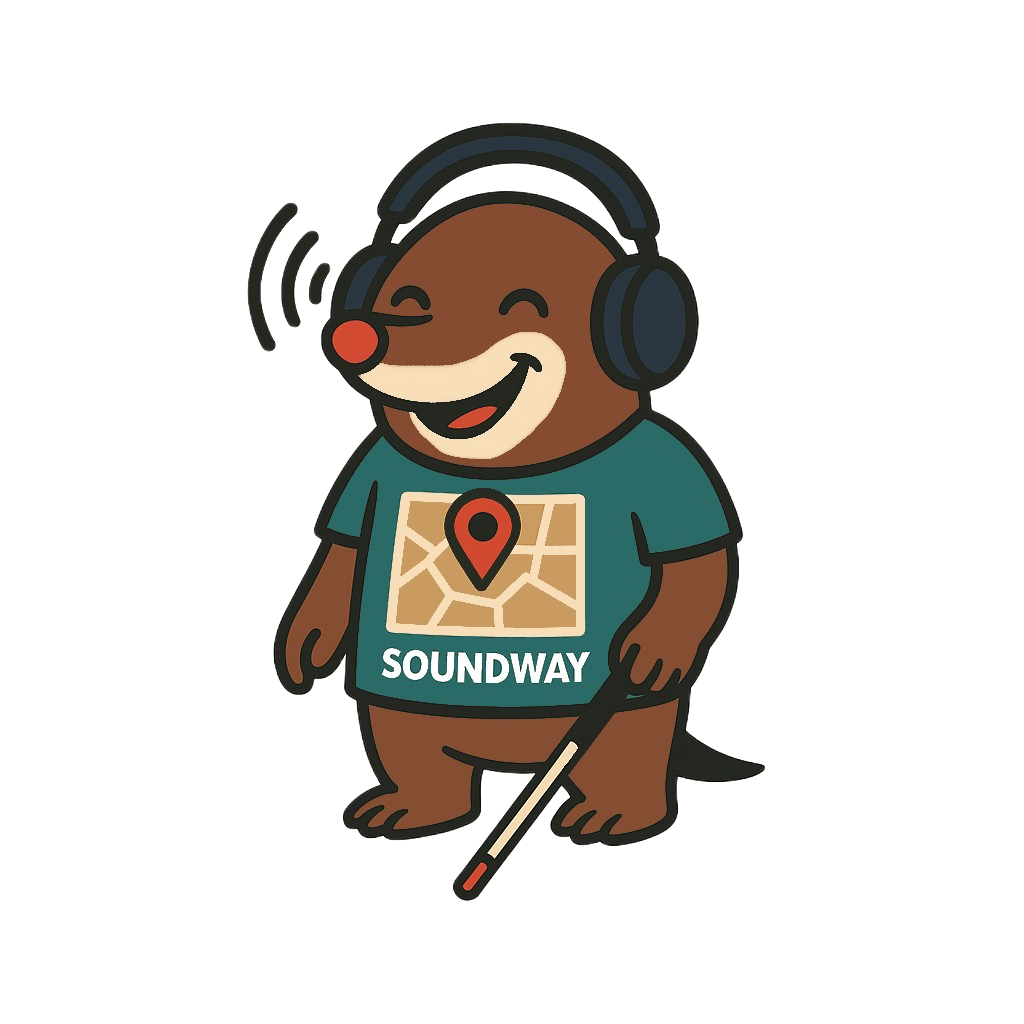
\includegraphics[width=0.32\textwidth]{figures/SoudWayLogo2.png}\\[0.5em]
    \textit{Logo of the SoundWay mobile application}
\end{center}

\begin{center}
    \vspace*{1em}
    
\includegraphics[width=0.32\textwidth]{figures/GetItOnGooglePlay_Badge_Web_color_French.png}\\
    \textit{(Early access planned on Google Play)}
\end{center}
% =====================================

\vspace*{2em}

\begin{center}
    
\includegraphics[width=1\textwidth]{figures/overview.pdf}\\
    \textit{(Global overview of the SoundWay system)}    
\end{center}

\vfill

\pagebreak
\tableofcontents
\pagebreak


% ===============================
\section{Preamble}
% ===============================

\index{Introduction}This document is the official user guide for \textbf{SoundWay}, an indoor orientation assistance system primarily intended for people with visual impairments.  
SoundWay was developed as part of the course \textbf{INFO M435 -- Embodied and Augmented Interfaces} at the University of Namur.

The system combines several components:
\begin{itemize}
    \item a \textbf{BLE multi-advertising emitter} based on a Raspberry Pi,
    \item a \textbf{mobile application} (smartphone) that receives and interprets BLE signals,
    \item a \textbf{voice interface} enabling hands-free interactions,
    \item \textbf{audio and vibratory feedback} guiding the user.
\end{itemize}

The purpose of this guide is to provide a clear, step-by-step description of:
\begin{itemize}
    \item system installation (Raspberry Pi + mobile application),
    \item minimal configuration and hardware prerequisites,
    \item the behaviour of the main functionalities,
    \item how to use SoundWay in indoor navigation scenarios.
\end{itemize}

\subsection{Introduction}
\index{Getting started}SoundWay is an augmented navigation prototype that uses \textit{Bluetooth Low Energy} (BLE) technology to help the user locate themselves and move within a building (for example, the Faculty of Computer Science at UNamur).  

The system relies on:
\begin{itemize}
    \item BLE multi-advertising signals emitted by a Raspberry Pi,
    \item distance estimation based on RSSI (received signal strength),
    \item an Android mobile application providing audio and vibratory indications,
    \item voice commands enabling the user to request help or directions.
\end{itemize}

This guide explains:
\begin{itemize}
    \item how to start the system,
    \item how to use the mobile interface,
    \item how to interpret voice messages and haptic feedback,
    \item several typical usage scenarios.
\end{itemize}

\subsection{What is this software?}

SoundWay is an \textbf{experimental indoor orientation platform} that combines sensing, wireless communication and voice interaction.  
It is not a simple interactive map, but a system that aims to \textbf{enhance the user’s perceptual abilities} by providing spatial cues through sound and vibration.

\subsubsection{Its objective}

The main objective of \textbf{SoundWay} is to facilitate navigation in indoor spaces (corridors, rooms, intersections) for people with reduced or no vision. More specifically, the system aims to:
\begin{itemize}
    \item provide simple proximity-based guidance (closer / farther),
    \item avoid dependence on heavy or expensive infrastructure,
    \item illustrate the potential of embodied and multimodal interaction (audio + haptics + movement).
\end{itemize}

\subsubsection{Main features}

\begin{itemize}
    \item \textbf{BLE multi-advertising emission}:  
    a Raspberry Pi broadcasts multiple BLE advertisements under a shared identifier (e.g. \texttt{King375}) in order to increase signal density.
    \item \textbf{BLE scanning and distance estimation}:  
    the smartphone continuously measures the RSSI and estimates the relative distance to the emitter.
    \item \textbf{Voice interface}:  
    the user can issue voice commands (e.g. “start guidance”, “repeat instruction”).
    \item \textbf{Audio and vibratory feedback}:  
    depending on the distance, the system produces sounds and/or vibrations that are more or less frequent or intense.
    \item \textbf{Simplified graphical interface}:  
    the screen displays minimal information (BLE connection status, estimated distance, microphone button).
\end{itemize}

\subsubsection{What SoundWay is not}

\paragraph{Not a full GPS}
SoundWay does not provide \textit{detailed mapping} or complex route computation. It mainly indicates the proximity of a point of interest (the emitter) and a few simple directional hints.

\paragraph{Not a certified medical device}
SoundWay is an academic prototype. It does not replace certified assistive technologies nor the human support required in some situations of visual impairment.

\paragraph{Not a tracking system}
The system does not track user movements and does not store trajectories. It only measures BLE signal strength locally on the smartphone.

\paragraph{Not a document storage system}
SoundWay does not store or manage files or documents. Its focus is orientation.

\subsubsection{Target audience}

\paragraph{Knowledge and user profiles}

This guide is intended for:
\begin{itemize}
    \item \textbf{end users} (people with visual impairments and their assistants) who wish to test the system in a controlled environment,
    \item \textbf{students} and researchers in human–computer interaction interested in embodied interaction,
    \item \textbf{developers} and \textbf{technicians} who want to install or adapt the system.
\end{itemize}

No extensive technical background is required for basic use. A minimal familiarity with Android smartphones and Bluetooth connectivity is nevertheless recommended.

\subsubsection{Usage licence}

The \textbf{SoundWay prototype} is distributed in an academic context, for teaching, experimentation and demonstration purposes. Unless otherwise specified in the code repository:

\paragraph{Attribution}
Any reuse must clearly acknowledge the \textbf{SoundWay} project and its authors (INFO M435 student group, University of Namur).

\paragraph{Non-commercial use}
The software is not intended for commercial use without explicit agreement from the authors and the University of Namur.

\paragraph{No warranty}
The system is provided “as is”, without any warranty. The authors cannot be held liable for any damage or loss resulting from its use.

% ===============================
\subsection{Legal notices}
% ===============================

\paragraph{Privacy and data processing}
\index{Privacy}SoundWay neither collects nor stores personal data on a remote server. All measurement data (RSSI, estimated distance) are processed \textbf{locally} on the smartphone.

\paragraph{Stored data}
Depending on the configuration, the mobile application may store:
\begin{itemize}
    \item a small number of local parameters (e.g. distance thresholds, language choice),
    \item technical logs useful for debugging, stored on the device.
\end{itemize}
These data are not transmitted to third-party services.

\paragraph{Liability}
The authors of SoundWay cannot be held responsible for:
\begin{itemize}
    \item incorrect or inappropriate use of the system,
    \item navigation decisions taken solely on the basis of the indications provided by the prototype,
    \item any measurement errors linked to the environment (obstacles, interference, etc.).
\end{itemize}

\paragraph{Technical limitations}
BLE technology is sensitive:
\begin{itemize}
    \item to physical obstacles (walls, furniture),
    \item to moving people,
    \item to the orientation of the smartphone and the user.
\end{itemize}
The indications provided by SoundWay are therefore always \textbf{approximate}.

\newpage
% ===============================
\section{How to install it?}
% ===============================

SoundWay installation is divided into two parts:
\begin{enumerate}
    \item preparation of the BLE emitter (Raspberry Pi),
    \item installation of the mobile application on the smartphone.
\end{enumerate}

\subsection{Hardware prerequisites}

\begin{itemize}
    \item \textbf{Raspberry Pi} (model 3B, 3B+ or 4, with integrated Bluetooth),
    \item power supply and microSD card (16 GB recommended),
    \item optionally a \textbf{USB Bluetooth dongle} for improved stability,
    \item an \textbf{Android smartphone} (Android 10 or later) with Bluetooth,
    \item \textbf{earphones} or a headset (ideally).
\end{itemize}

\subsection{Installation on the Raspberry Pi}

\paragraph{1. Install the operating system}
Install \textit{Raspberry Pi OS} (or an equivalent distribution) on the microSD card using the official imaging tool.

\begin{figure}[h]
    \centering
    \includegraphics[width=0.6\textwidth]{figures/placeholder-rpi-imager.png}
    \caption{(Screenshot placeholder) Selection of the Raspberry Pi OS image in the SD card imaging tool.}
    \label{fig:rpi_imager}
\end{figure}

\paragraph{2. Enable Bluetooth}
Once the Raspberry Pi has booted:
\begin{itemize}
    \item ensure that Bluetooth is enabled,
    \item update the system:
\begin{verbatim}
sudo apt update
sudo apt upgrade
\end{verbatim}
\end{itemize}

\paragraph{3. Install BLE dependencies}

Install the required packages (BlueZ, D-Bus, Python and associated libraries):
\begin{verbatim}
sudo apt install bluetooth bluez python3 python3-pip
\end{verbatim}

\paragraph{4. Retrieve the SoundWay code}

Clone the repository (or copy the project files) into a directory, for example:
\begin{verbatim}
git clone <SOUNDWAY_REPOSITORY_URL>.git
cd SoundWay/raspberry
pip3 install -r requirements.txt
\end{verbatim}

\paragraph{5. Start the BLE emitter}

Run the advertising script (indicative name):
\begin{verbatim}
python3 soundway_advertiser.py
\end{verbatim}

You should see terminal messages indicating that multiple BLE advertisements are being broadcast under the shared identifier (e.g. \texttt{King375}).

\begin{figure}[h]
    \centering
    \includegraphics[width=0.9\textwidth]{figures/placeholder-rpi-terminal.png}
    \caption{(Screenshot placeholder) Raspberry Pi terminal showing the SoundWay script running.}
    \label{fig:rpi_terminal}
\end{figure}

\newpage
\subsection{Installing the mobile application}

\paragraph{1. Enable unknown sources (if using an APK)}

If the application is provided as an \texttt{.apk} file:
\begin{itemize}
    \item copy the file to the smartphone,
    \item if necessary, enable installation from unknown sources,
    \item launch the APK installation.
\end{itemize}

\paragraph{2. First launch}

At first start-up, the SoundWay application will request:
\begin{itemize}
    \item permission to use \textbf{Bluetooth},
    \item access to \textbf{location} (required for BLE scanning on Android),
    \item optionally access to the \textbf{microphone} for voice recognition.
\end{itemize}

\begin{figure}[h]
    \centering
    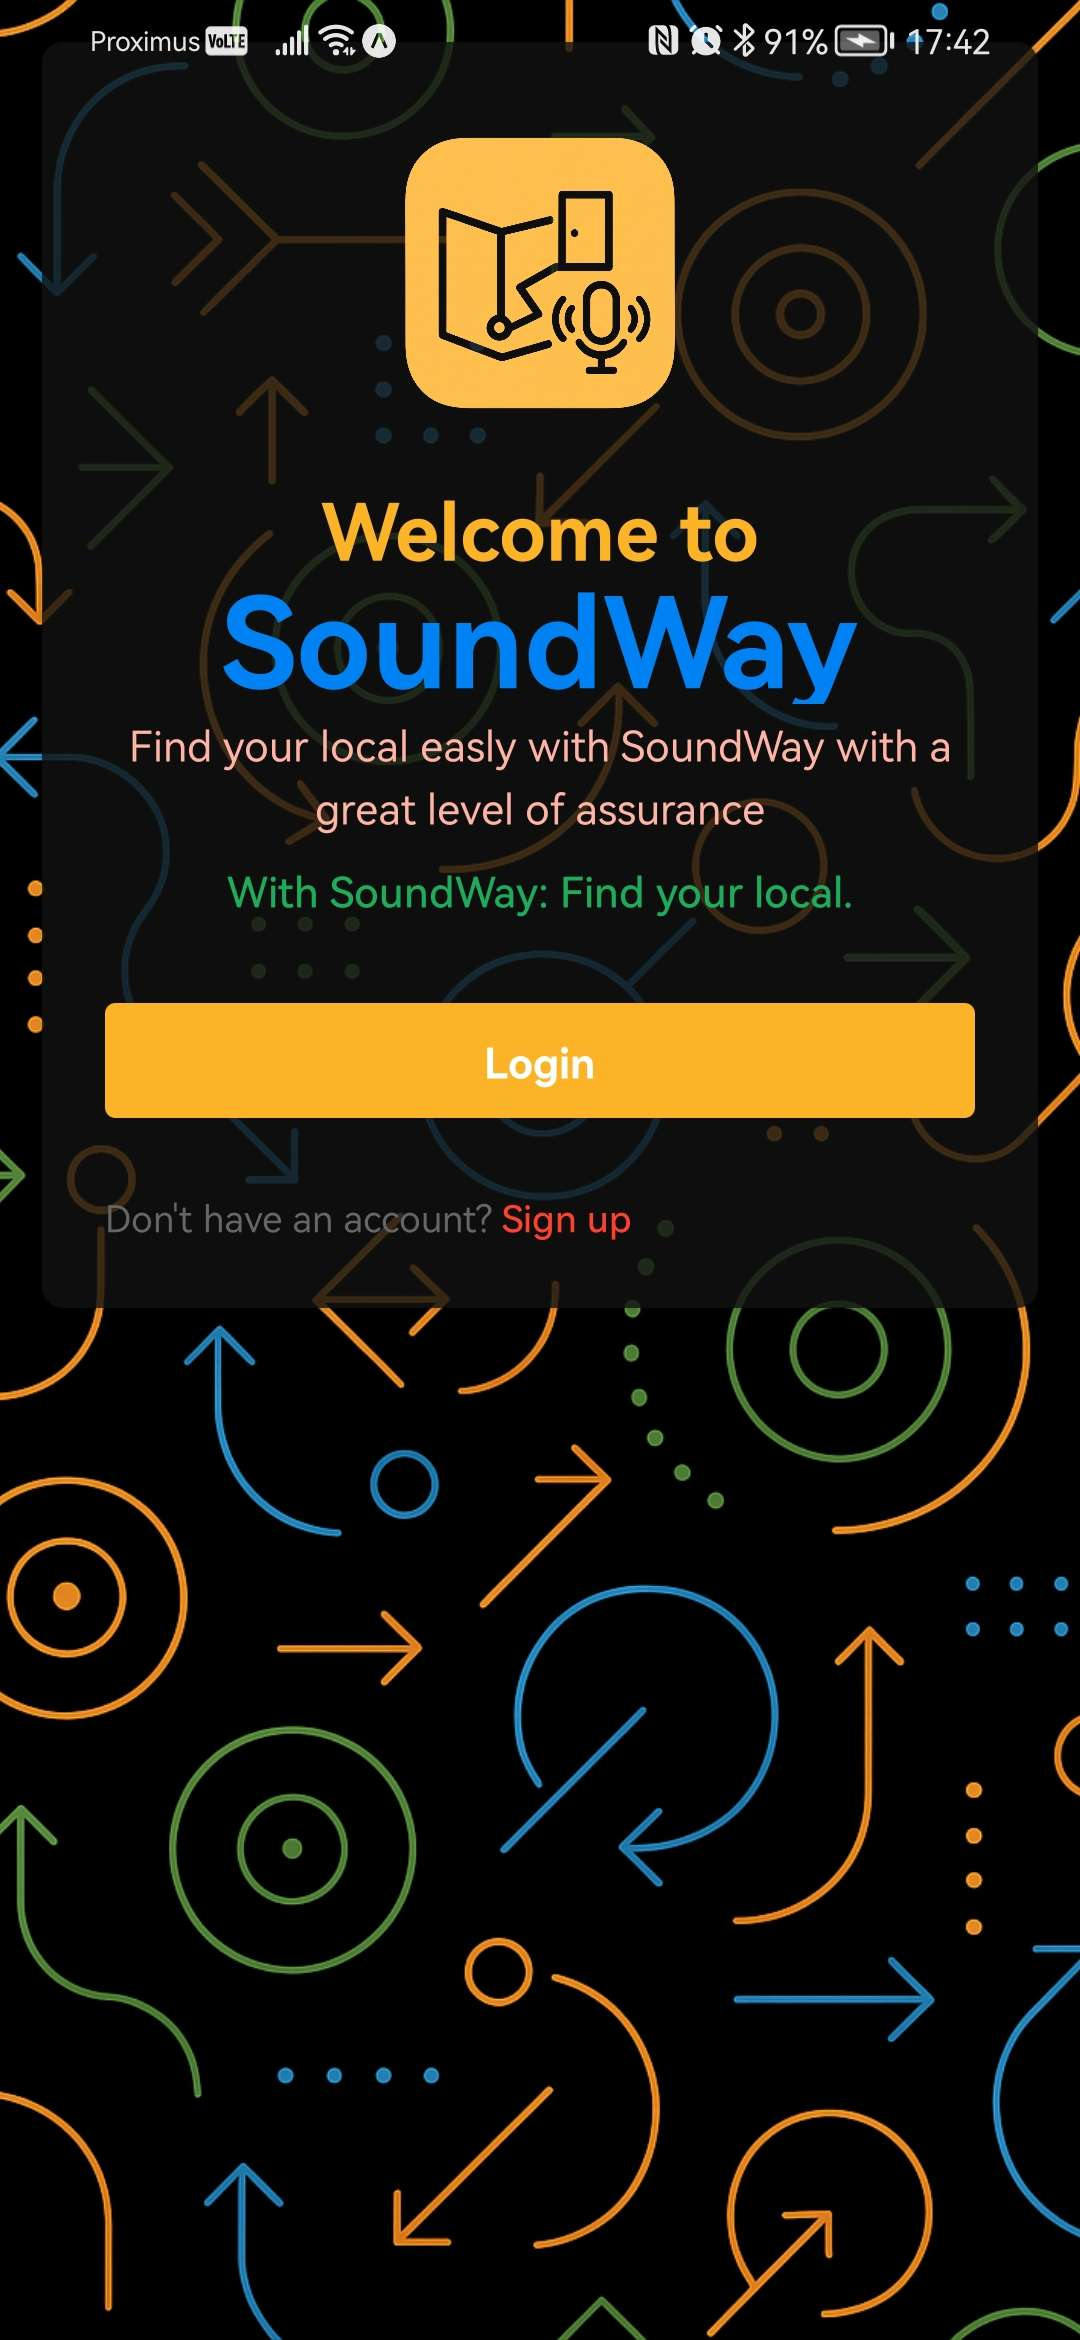
\includegraphics[width=0.28\textwidth]{figures/soundway-login.jpg}
    \caption{Welcome / permissions screen of the SoundWay application (example).}
    \label{fig:app_permissions}
\end{figure}

\paragraph{3. Minimal configuration}

From the main screen, the user (or an assistant) can check:
\begin{itemize}
    \item the Bluetooth status (enabled / disabled),
    \item whether microphone access is enabled (for the voice interface),
    \item the name or identifier of the point of interest (e.g. \texttt{King375}).
\end{itemize}

% ===============================
\subsection{Supported operating systems}
% ===============================

\textbf{Raspberry Pi}: Raspberry Pi OS (or equivalent Linux distribution with BlueZ)  
\textbf{Smartphone}: Android 10+ (tested on a recent Android smartphone)

No external server installation is required: the system operates entirely locally (Raspberry Pi + smartphone).

\newpage
% ===============================
\section{How to use it?}
% ===============================

This section presents the main screens of the mobile application and explains how to use SoundWay in a typical orientation scenario.

\subsection{Overview of functionalities}

\subsubsection{Main screen}

The main screen generally displays:
\begin{itemize}
    \item an indicator of BLE connection status,
    \item the estimated distance to the emitter (in metres or proximity levels),
    \item a button to activate the microphone (voice command),
    \item optionally a mode indicator (guidance active / inactive).
\end{itemize}

\begin{figure}[h]
    \centering
    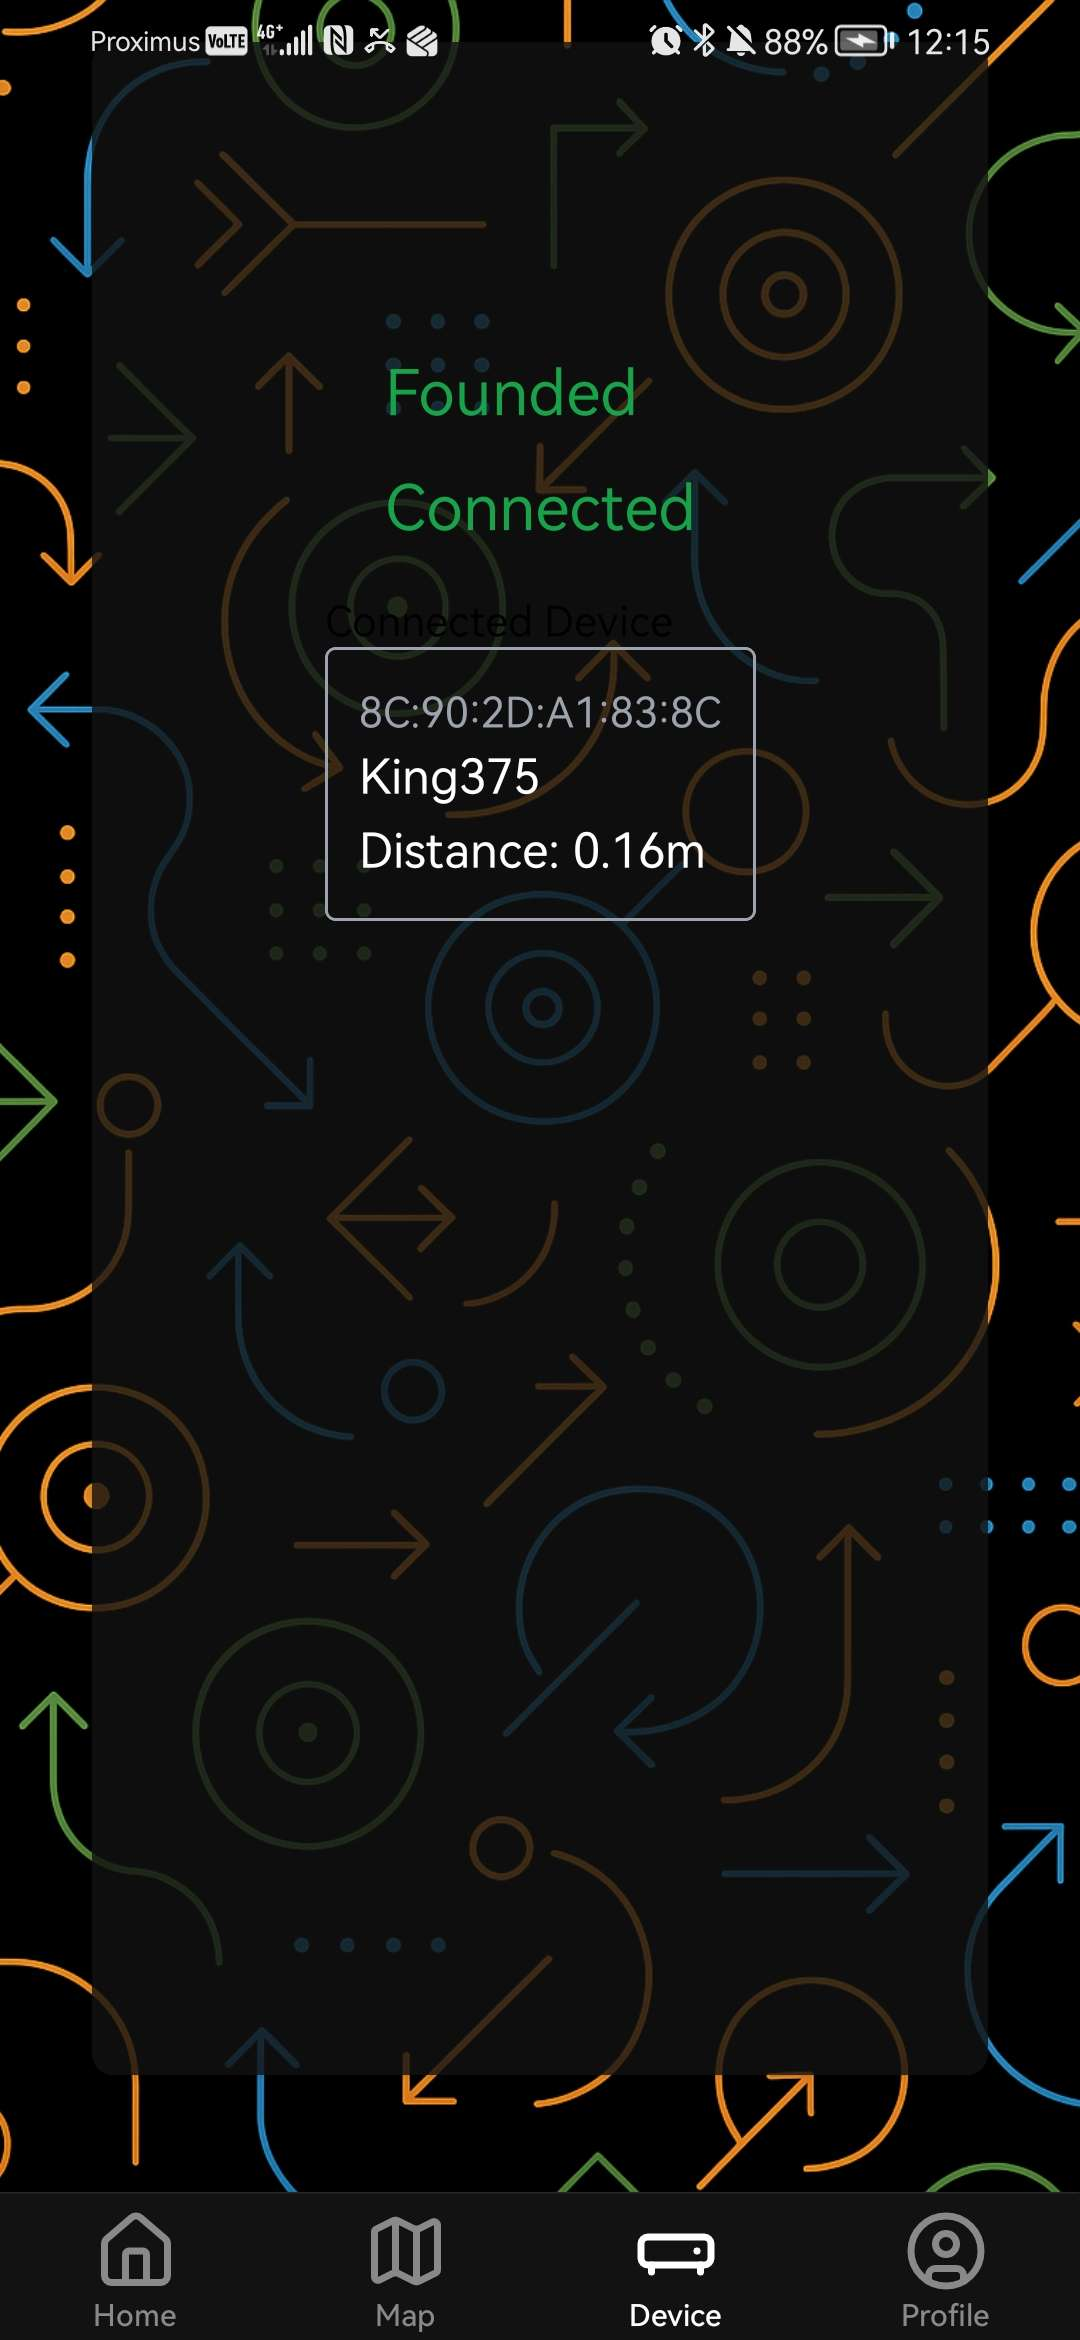
\includegraphics[width=0.28\textwidth]{figures/soundway-distance.jpg}
    \caption{Distance feedback screen of the SoundWay application.}
    \label{fig:app_distance}
\end{figure}

\subsubsection{Voice interface}

The application includes a \textbf{microphone} button to issue a voice command.  
Examples of commands (depending on the prototype configuration):
\begin{itemize}
    \item “\textit{Start guidance}”
    \item “\textit{Stop guidance}”
    \item “\textit{Repeat instruction}”
\end{itemize}

When the microphone is active, the smartphone sends the command to the voice recognition module and then displays or announces the response.

\begin{figure}[h]
    \centering
    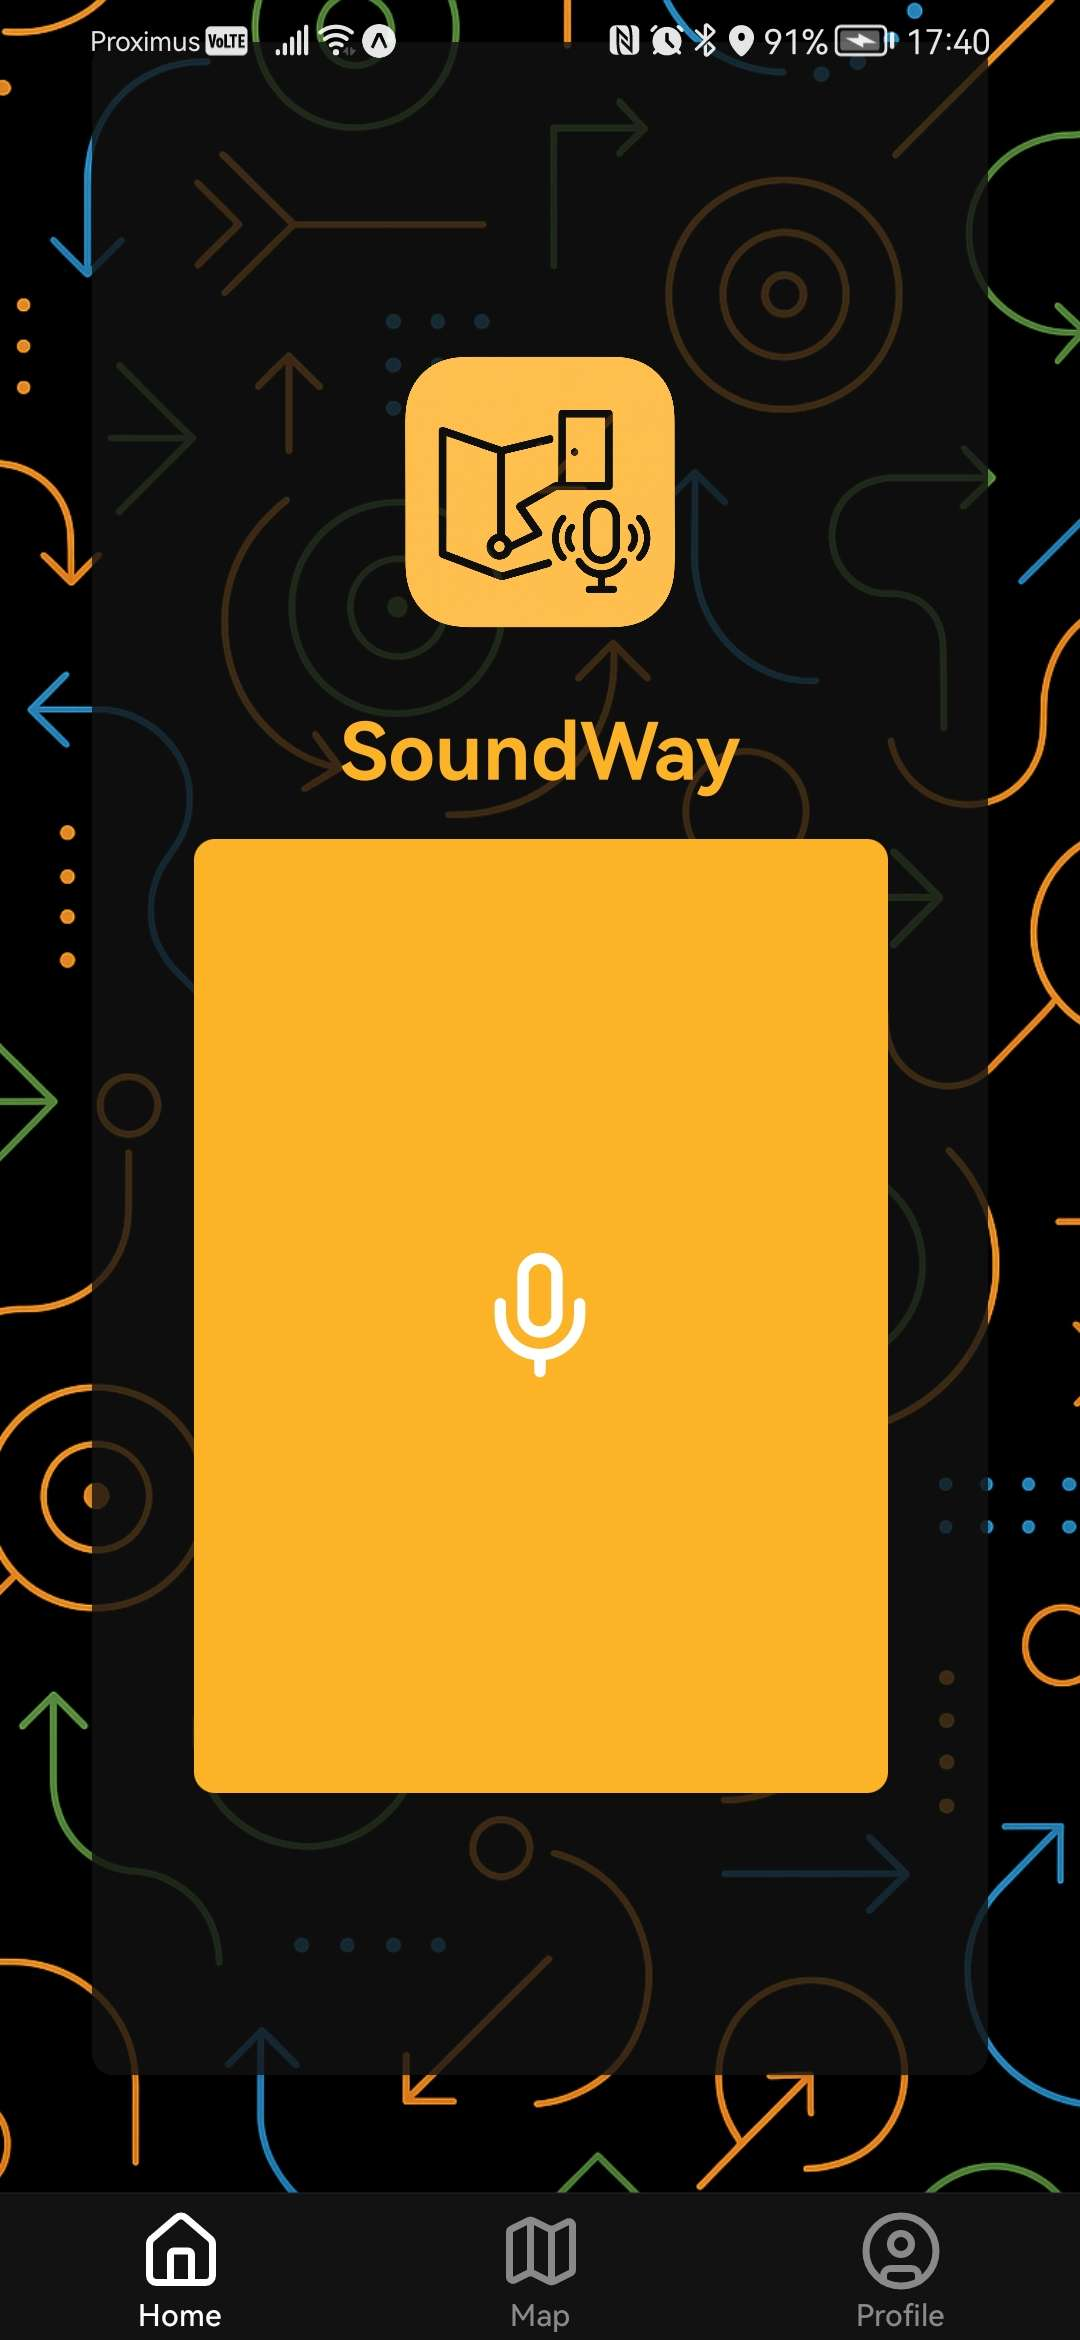
\includegraphics[width=0.28\textwidth]{figures/soundway-voice.jpg}
    \caption{Voice interaction screen: microphone activated to control SoundWay.}
    \label{fig:app_voice}
\end{figure}

\subsubsection{Audio and vibratory feedback}

Depending on the estimated distance, SoundWay may:

\begin{itemize}
    \item emit \textbf{beeps} at varying rates,
    \item make the smartphone vibrate more strongly as the user gets closer,
    \item produce verbal indications (e.g. “you are getting closer”, “you are moving away”).
\end{itemize}

The aim is to provide a \textbf{continuous interaction loop} between:
\begin{enumerate}
    \item the user’s movement,
    \item the perceived BLE signals,
    \item the audio and haptic feedback.
\end{enumerate}

\newpage
\subsection{Quick start guide}

\paragraph{Steps for the end user}

\begin{enumerate}
    \item Verify that the \textbf{Raspberry Pi} is powered on and that the BLE advertising script is running.
    \item On the \textbf{smartphone}, enable Bluetooth (and location if requested).
    \item Launch the \textbf{SoundWay} application.
    \item Check that the application detects the emitter (a message such as “beacon detected” may appear).
    \item Press the \textbf{Start guidance} button or use the corresponding voice command.
    \item Walk slowly along the corridor or test area and listen to the feedback:
    \begin{itemize}
        \item if beeps become faster and vibrations more frequent, you are getting closer,
        \item if feedback becomes less frequent, you are moving away.
    \end{itemize}
    \item Once close to the target point, the application may indicate arrival (“you have reached your destination”).
\end{enumerate}

\subsection{Use cases}

\subsubsection{Example: Reaching an information point in a corridor}

\begin{itemize}
    \item Place the Raspberry Pi near the information point (e.g. at the entrance of a room).
    \item Launch the SoundWay application in the corridor.
    \item Activate guidance mode.
    \item Walk slowly and adjust your trajectory according to the audio feedback (stronger when approaching).
\end{itemize}

\begin{figure}[h]
    \centering
    \includegraphics[width=0.45\textwidth]{figures/placeholder-user-walk.png}
    \caption{(Screenshot placeholder) User equipped with SoundWay walking towards the beacon.}
    \label{fig:user_walking}
\end{figure}

\subsubsection{Example: Use with human assistance}

In an experimental context, the visually impaired user may be accompanied by a sighted person:
\begin{itemize}
    \item the assistant checks Bluetooth status and permissions,
    \item then lets the user explore the space relying on audio and haptic feedback,
    \item the assistant remains ready to intervene in case of danger or obstacles.
\end{itemize}

\newpage
\subsection{Troubleshooting}

\paragraph{Unable to detect the BLE beacon}
\begin{itemize}
    \item Check that the Raspberry Pi is powered on.
    \item Verify that the \texttt{soundway\_advertiser.py} script is running (see terminal).
    \item Ensure that Bluetooth is enabled on the smartphone.
    \item Move physically closer to the beacon (initially within 5 metres).
\end{itemize}

\paragraph{Unstable signal or strongly fluctuating distance}
\begin{itemize}
    \item Check that there are not too many obstacles between you and the beacon.
    \item Try holding the smartphone in a stable position (for example in front of you).
    \item Avoid standing directly behind a wall or large metallic object.
\end{itemize}

\paragraph{Voice commands not working}
\begin{itemize}
    \item Verify that microphone access is enabled for the SoundWay application.
    \item Reduce ambient noise if possible.
    \item Speak at a normal volume and articulate clearly.
\end{itemize}

\paragraph{Application crashes or displays an error}
\begin{itemize}
    \item Restart the SoundWay application.
    \item If the problem persists, reboot the smartphone.
    \item If possible, note the error message and the context (to assist the development team).
\end{itemize}

\newpage
% ===============================
\section{Frequently Asked Questions (FAQ)}
% ===============================

\subsection{Installation and configuration}

\begin{itemize}
    \item \textbf{Q: Do I need an Internet connection to use SoundWay?}\\
    A: No. Everything operates locally (Raspberry Pi + smartphone).

    \item \textbf{Q: What type of smartphone is required?}\\
    A: An Android smartphone with Bluetooth Low Energy (BLE) and Android 10+ is recommended.

    \item \textbf{Q: Can I move the beacon (Raspberry Pi)?}\\
    A: Yes, but you may need to recalibrate the test area or inform users of the new position.

    \item \textbf{Q: Is there an iOS application?}\\
    A: Not in the current version of the prototype (Android only).
\end{itemize}

\subsection{General use}

\begin{itemize}
    \item \textbf{Q: Does the application provide a map of the building?}\\
    A: No. SoundWay provides proximity indications and audio/haptic feedback, but not a detailed map.

    \item \textbf{Q: Can the system manage multiple beacons?}\\
    A: The prototype focuses on a single main emitter. A multi-beacon deployment would require more advanced configuration.

    \item \textbf{Q: Does SoundWay work in any building?}\\
    A: In principle yes, but performance strongly depends on the architecture (walls, materials, interference).
\end{itemize}

\newpage
% ===============================
\section{Glossary}
% ===============================

\begin{description}
    \item[BLE (Bluetooth Low Energy)] Bluetooth technology with low energy consumption, used for beacons and proximity communications.

    \item[RSSI] \textit{Received Signal Strength Indicator}. Measurement of received signal power. SoundWay uses it to estimate the relative distance to the beacon.

    \item[Multi-advertising] Technique consisting in broadcasting multiple BLE advertisements simultaneously to increase detection frequency and robustness.

    \item[Raspberry Pi] Single-board microcomputer used here as a BLE emitter.

    \item[Haptic guidance] Use of vibrations (or other physical feedback) to convey information to the user.

    \item[Voice interaction] Interaction via speech, including voice commands (input) and speech synthesis (output).
\end{description}

\newpage
% ===============================
\section{Bibliography}
% ===============================

\subsection{Further reading}

\begin{thebibliography}{9}

\bibitem{engelbart1962}
Douglas Engelbart.  
\textit{Augmenting Human Intellect: A Conceptual Framework}.  
Stanford Research Institute, 1962.

\bibitem{dix2004}
Alan Dix et al.  
\textit{Human–Computer Interaction}.  
3rd Edition, Pearson, 2004.

\bibitem{preece2015}
Jennifer Preece, Yvonne Rogers, Helen Sharp.  
\textit{Interaction Design: Beyond Human–Computer Interaction}.  
4th Edition, Wiley, 2015.

\bibitem{blebook}
Robin Heydon.  
\textit{Bluetooth Low Energy: The Developer’s Handbook}.  
Prentice Hall, 2012.

\end{thebibliography}

\subsection{References on navigation and accessibility}

\begin{thebibliography}{9}

\bibitem{kammoun2012}
Samir Kammoun et al.  
\textit{Navigation and Space Perception for Blind People}.  
Journal of Assistive Technologies, 2012.

\bibitem{mekhalfi2016}
Mekhalfi et al.  
\textit{Recovering the Sight of the Blind: An Overview of the Research}.  
IEEE Signal Processing Magazine, 2016.

\end{thebibliography}

\newpage
% ===============================
\section{Appendix}
% ===============================

\subsection{Appendix A: Suggested screenshots}

The following locations are reserved for real screenshots of the SoundWay application:

\begin{itemize}
    \item Welcome / permissions screen (Fig.~\ref{fig:app_permissions}),
    \item Voice interaction screen (Fig.~\ref{fig:app_voice}),
    \item Distance and guidance screen (Fig.~\ref{fig:app_distance}),
    \item Photograph of the user during a test session (Fig.~\ref{fig:user_walking}),
    \item Raspberry Pi terminal displaying multi-advertising (Fig.~\ref{fig:rpi_terminal}),
    \item SD card flashing tool (Fig.~\ref{fig:rpi_imager}).
\end{itemize}

\subsection{Appendix B: Possible evolutions}

Planned evolutions for SoundWay include:
\begin{itemize}
    \item management of \textbf{multiple beacons} within the same building,
    \item integration of \textbf{simplified maps} or \textbf{landmarks},
    \item improvement of RSSI filtering algorithms (Kalman filter, adaptive moving average),
    \item customisation of feedback profiles (more or fewer sounds, more or fewer vibrations, etc.).
\end{itemize}

\bigskip
\hrule
\bigskip

{\small \noindent © 2025 Authors of SoundWay.\\
    This document is distributed under the terms of the Creative Commons CC BY-ND (Attribution - No Derivatives) licence. \doclicenseThis}

\bigskip
\hrule

\printindex

\end{document}
